\section{Triangles}


\begin{defn}[The Law Of Cosines \label{defn:Law Of Cosines}]{1}
\keyword{The Law of Cosines} relates the side lengths of a triangle to the cosine of one of its angles. For a triangle with side lengths $a$, $b$, and $c$, and angle $C$ opposite to side $c$, the Law of Cosines is given by:
\begin{center}
\begin{minipage}{0.3\linewidth}
	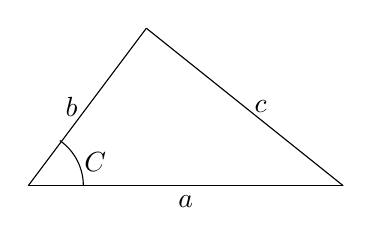
\begin{tikzpicture}
		% Triangle vertices
		\coordinate (A) at (0,0);
		\coordinate (B) at (4,0);
		\coordinate (C) at (1.5,2);
		
		% Triangle sides
		\draw (A) -- (B) node[midway,below] {$a$};
		\draw (B) -- (C) node[midway,right] {$c$};
		\draw (C) -- (A) node[midway,left] {$b$};
		
		% Angle C
		\draw (0.7,0) arc (0:55:0.7);
		\node at (0.85,0.3) {$C$};
	\end{tikzpicture}
\end{minipage}
\begin{minipage}{0.4\linewidth}
	\begin{align}
		c^2 = a^2 + b^2 - 2ab\cos C
	\end{align}
\end{minipage}
\end{center}
\end{defn}

Notice from definition \ref{defn:Law Of Cosines} that if the angle $C = 90^\circ = \pi/2$, then the cosine term would evaluate to zero and we'd be left with \keyword{the Pythagorean theorem} $c^2 = a^2 + b^2$.
